\chapter{Schnittstellen}


Lorem ipsum dolor sit amet, consectetur adipiscing elit. Sed gravida mollis placerat. Sed congue iaculis massa vitae dapibus. Fusce sed felis lorem. Suspendisse purus diam, sollicitudin vitae imperdiet ac, placerat eu metus. In luctus, metus vel dictum hendrerit, diam lacus cursus enim, eu porta augue lacus non metus. Pellentesque habitant morbi tristique senectus et netus et malesuada fames ac turpis egestas. Nullam nec orci eget metus pulvinar sagittis. Vestibulum ante ipsum primis in faucibus orci luctus et ultrices posuere cubilia Curae; Sed turpis lorem, aliquet eu ornare non, viverra ac urna.

\section{Server TourLive Schnittstelle}

Praesent libero lectus, ultrices eget pharetra sed, sollicitudin et est. Pellentesque quis urna eget lorem sodales venenatis eget nec quam. In sagittis aliquam auctor. Phasellus vitae ipsum purus, sit amet imperdiet nunc. Pellentesque habitant morbi tristique senectus et netus et malesuada fames ac turpis egestas. Ut malesuada nibh ut lectus scelerisque sed iaculis lectus varius. Nulla blandit turpis tortor. Nulla facilisi. Cum sociis natoque penatibus et magnis dis parturient montes, nascetur ridiculus mus. Nam leo ante, porta vel scelerisque at, volutpat eu sapien. Aliquam viverra adipiscing sapien et porta. Sed quis diam ut sem tincidunt consectetur varius non dolor. Fusce fermentum, quam vitae suscipit euismod, leo erat malesuada ante, ac consequat est lacus eget enim. Proin lacinia justo et est vehicula adipiscing rhoncus lacus mollis.

\section{Devicemanagement Schnittstelle}

Für alle Funktionen, auf die von dem Aufnahmesystem her zugegrifen werden, steht eine JSON Schnittstelle mit URL zur Verfügung. Im folgenden werden diese näher beschrieben.

\subsection{Status posten und Einstellungen erhalten}

Um den aktuellen Status des Aufnahmesystems dem Server mitzuteilen kann diese Methode aufgerufen werden. Als Antwort erhält man die im Moment aktuellen Einstellungen.

{\bf URL: }http://tlng.cnlab.ch/devmgmtsrv/api/getdevicemanagementcontainer 

\subsubsection{Status JSON}

Das JSON eines Status Posts sieht folgendermassen aus:

\begin{figure}[h]
	\centering
	\caption{Status JSON}
	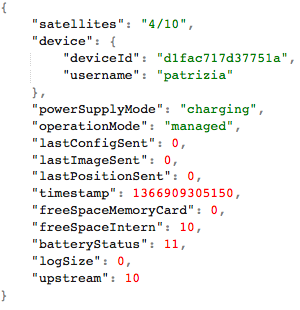
\includegraphics[height=80mm]{images/StatusJson.png}
\end{figure}


\subsubsection{Einstellungen JSON}

Die Antwort die man bei dieser Anfrage erhält ist die folgende:

\begin{figure}[H]
	\centering
	\caption{Einstellungen JSON}
	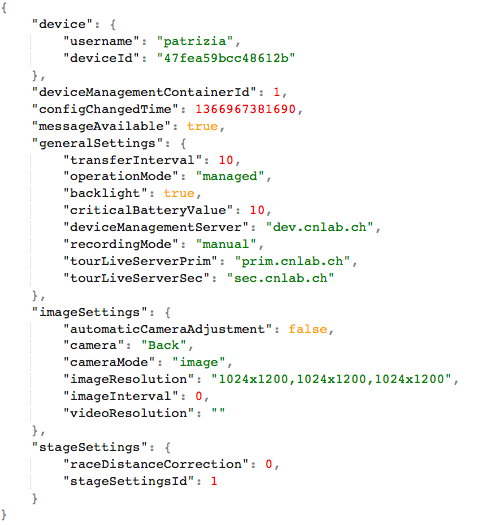
\includegraphics[height=120mm]{images/SettingsJson.png}
\end{figure}


\subsection{Log posten}

Um neue Logeinträge dem Server zu übermitteln kann diese Methode benutzt werden.

{\bf URL: }http://tlng.cnlab.ch/devmgmtsrv/api/postlog

\subsubsection{Log JSON}

Das JSON eines Log Posts sieht folgendermassen aus:

\begin{figure}[H]
	\centering
	\caption{Log JSON}
	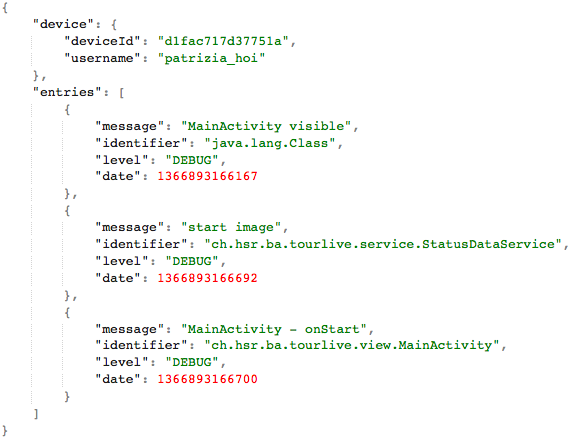
\includegraphics[height=100mm]{images/LogJson.png}
\end{figure}

\subsection{Nachricht abholen}

Sofern eine neue Nachricht für das Gerät vorhanden ist kann sie über diese Methoden abgeholt werden.

{\bf URL: }http://tlng.cnlab.ch/devmgmtsrv/api/getmsg/{deviceId}

\begin{figure}[H]
	\centering
	\caption{Nachricht JSON}
	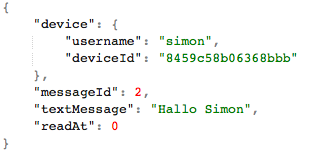
\includegraphics[height=30mm]{images/MessageJson.png}
\end{figure}


